\documentclass{article}
\usepackage[utf8]{inputenc}
\usepackage[a4paper, total={6in, 10in}]{geometry}
\usepackage{fancyhdr}
\usepackage{hyperref}
\usepackage{csquotes}
\usepackage{graphicx}
\usepackage[skip=10pt]{caption}
\usepackage[square]{natbib}
\setcitestyle{numbers}

%%% COVER PAGE
\title{\textbf{Chaos Engineering}}
\author{
    Anders Eriksson \\ \url{aeri3@kth.se}
    \and
    Lukas Szerszen \\ \url{lukassz@kth.se}
}

%%% HEADER
\pagestyle{fancy}
\lhead{Anders Eriksson \& Lukas Szerszen}
\rhead{Chaos Engineering}

%%% DOCUMENT
\begin{document}

\maketitle

\section{Introduction}
Program code which deals which faults and failures is part of every system. The purpose of these routines is to quickly recover the system state such that the disruption in service is as small as possible. Outages not only affect the user's experience, but cost businesses millions with one-third of companies reporting that just an hour of downtime can cost between \$1 to \$5 million \cite{GremlinPaper}. With businesses now building their systems with microservices and on a distributed cloud architecture, the complexity has reached a point where failure scenarios have become much harder to predict \cite{chaosEngineeringGremlin}. As such,
due to the fragility of services and the possibility of  failure at any time in a distributed system, there is an increased emphasis on monitoring and fault-handling code \cite{GremlinPaper}\cite{microserivces}. However, it is has been the case that in classical operations, recovery code is not frequently executed in a production environment. As a result, there can be little confidence in failure and fault handling code that is grounded in actual experience gained from production \cite{GremlinPaper}\cite{introductionToChaos}.

To build a grounded understanding of the system's resilience, developers have begun to employ an approach which continuously causes the system to execute its error handling and fault recovery code in production. This approach is based around injecting faults into the system that induce failures  \cite{GremlinPaper}. By injecting faults in a controlled and planned out manner, the developers and operations teams can asses the error-handling procedures in a production environment. This leads to an increased knowledge about the system, and also helps to discover and most importantly fix potentially unexpected errors. This emergent practice has come to be known as \textit{Chaos Engineering} \cite{GremlinPaper}.

Chaos Engineering is a discipline in which thoughtful and planned experiments are designed and carried out in order to reveal weaknesses in the system \cite{OreillyChaos}. The experiments are based on intentionally injecting failure into the system and their purpose is to learn about the system's vulnerabilities. It is important to emphasize the point that Chaos Engineering is not an ad hoc process where the purpose is to randomly break things. The process is based on continuous experimentation methods which enable for a scientific evaluation of the system \cite{OreillyChaos}. By carrying out experiments which expose weaknesses in a system, chaos engineers (or site reliability engineers) can amend issues prior to costly outages, thereby increasing the resilience  of the system \cite{OreillyChaos}.

With this as a premise, the purpose of this essay is to explore the area that is Chaos Engineering. We aim to look at the theoretical background of chaos engineering and present the core concepts and principles of it, but also the background for its emergence. In addition to this, we like to personally explore some of the chaos engineering technologies available today. We hope that this essay can serve as a readily available introduction to the area and some chaos engineering technologies.

\section{Background}
In today's IT-economy, many companies tailor their businesses such that they are always available on the internet \cite{GremlinPaper}\cite{introductionToChaos}. Alongside this development, the manner in which system's architecture is built and maintained has also changed. System architecture some years ago was primarily structured in a ``monolithic`` style \cite{microserivces}\cite{introductionToChaos}. The architecture was comprised in three tiers; a client-side user interface, a database running in a data center and a server-side application. Systems with this architecture ran in highly controlled environments, with knowledge and routines for the physical racks running their hosts \cite{GremlinPaper}\cite{introductionToChaos}.

While still a valid architecture, there has been a rapid shift to the cloud and developing software on a microservice architecture \cite{GremlinPaper}. In a microservice architecture, a single application is built as a suite of small, independent, but interconnected services. The services are modular and run a unique process which captures a specific business functionality. By communicating with one another, the services are able to deliver the full spectrum of business goals \cite{microserivces}\cite{GremlinPaper}. Supporting this architecture is a myriad of web server's data bases, load balancers, routers, monitors and more which have to work together in a coordinated fashion \cite{GremlinPaper}.

The adoption of a large-scale, modular and distributed architecture design enabled businesses to be more flexible with their development and deployment cycle \cite{principlesOfChaos}\cite{GremlinPaper}.
With distributed cloud architectures, new challenges emerged due to the increase in complexity of the infrastructure \cite{GremlinPaper}\cite{chaosEngineeringGremlin}. Businesses now rely upon other services which host their cloud-based applications, and as such have to deal with scenarios where a failure is outside of their direct control. Additionally, coordinating the interaction between all the components can lead to unpredictable outcomes; hard disks failing, a surge in customer traffic overloading a components, among others, lead to failures \cite{OreillyChaos}\cite{principlesOfChaos}. That is to say that, services can fail due to a myriad of reasons, at any time, which can lead to cascading effects in relation to other services in the system \cite{microserivces}\cite{principlesOfChaos}.The complexity has reached a level such that it is no longer feasible to predict all possible ways for such a system to fail \cite{GremlinPaper}\cite{OreillyChaos}.


\section{Chaos Engineering}
The term Chaos Engineering in of itself is new and the practice of it is still emerging \cite{OreillyChaos}. It is comprised of core concepts which define principles, which in turn guide the chaos methodology in practice \cite{chaosJVM}\cite{OreillyChaos}. The concepts which chaos engineering is based on are; \textit{perturbation, hypothesis, experiment, blast radius}.

A perturbation refers to the controlled and proactive injection of a fault which impacts the system's state, execution flow or environment \cite{chaosJVM}. These perturbations are also referred to as "chaos variables", and it is pertinent that they are representative of real world events such as; servers dying, connection time out etc \cite{chaosJVM}\cite{principlesOfChaos}.

A hypothesis is a educated guess of the expected outcome of injecting a perturbation on systemic behavior which is quantified and measured \cite{chaosJVM}\cite{OreillyChaos}. An example would be; by shutting down an entire AWS region, the traffic is expected to be diverted to other regions.

An experiment is the process of carrying out a planned out method which tests the hypothesis and deem whether the yielded results validate or falsify it. In chaos engineering, this is then equivalent of injecting the system with a perturbation and comparing the result with the hypothesis.

Lastly, there is the concept of a blast radius. It is important that experiments do not impact the system excessively, especially unnecessarily. As such, the blast radius defines the area of effect for the experiment. An experiment should not disturb behavior outside of the area \cite{chaosJVM}\cite{OreillyChaos}. An example of this is would be to start experiments in the staging environment, and eventually increasing it to  experiments running in production \cite{GremlinPaper}.

A key distinction between testing and chaos engineering, is that testing looks to assert a preconceived condition, given some inputs and conditions within the system, a specific output is expected. Similarly, fault injection is used for breaking the system in some preconceived way and asserting a condition. This differs from the core method of chaos engineering, which is experimentation for the purpose of gaining new knowledge about how a complex system may misbehave \cite{OreillyChaos}. That is to say that testing and failure injection in of themselves do not generate new information about the system \cite{OreillyChaos}. 

There are four principles which guide Chaos Engineering  in practice \cite{principlesOfChaos}:
\begin{enumerate}
    \item Start by defining ‘steady state’ as some measurable output of a system that indicates normal behavior.
    \item Hypothesize that this steady state will continue in both the control group and the experimental group.
    \item Introduce variables that reflect real world events like servers that crash, hard drives that malfunction, network connections that are severed, etc.
    \item Try to disprove the hypothesis by looking for a difference in steady state between the control group and the experimental group.
\end{enumerate}
The first step requires a a metric to be defined. This metric should identify and quantify the characteristics which represent a correct and steady state which exhibits the expected normal behavior \cite{chaosJVM}. Examples of metrics are the overall system's throughput, error rates, latency percentiles, stream starts per second etc \cite{principlesOfChaos}\cite{OreillyChaos}. As such metrics are not static but vary over time, it is necessary to reason about the steady state in terms of ranges of acceptable metric values. These ranges define the systemic behavior which is considered to be a baseline healthy system. A system who's metric values start to deviate outside the range(s) should be considered to no longer be in its steady state \cite{chaosJVM}. Secondly, the perturbations to be injected are defined \cite{chaosJVM}. Then, define a control and experimental phase (or group as stated in the principles). The control phase is there to monitor the steady state of the system, while in the experimental phase, the perturbation is injected and the effect monitored. These three steps are the preparatory steps required to perform a chaos engineering experiment. The last step is to carry out the experiment by injecting the perturbation into the system and monitoring the effect on the metrics defined \cite{chaosJVM}. Then by comparing the difference in the metrics between the control and experimentation phase, one evaluates the hypothesis. Either, the hypothesis is falsified and thereby a new issue has been discovered which must be reported and rectified. Or, the hypothesis is validated, which entails that there is a increased confidence in the resilience of the system which is grounded in actual experience \cite{chaosJVM}.

\section{Current State of the Art}
\label{sec:stateoftheart}

In this section, two state of the art chaos engineering technologies are presented. For our personal evaluation of our experiences testing the technologies presented in this section, please refer to section \ref{sec:discussion}. 

\subsection{Chaos Monkey}

Chaos Monkey is a resiliency tool created and maintained by Netflix that claims to follow the Principles of Chaos Engineering \cite{chaosmonkeyrepo}\cite{principlesOfChaos}. Originally part of the chaos engineering software suite named \textit{Simian Army} \cite{simianrepo}, a newer version was released as a standalone service in October 2016 \cite{chaosMonkeyUpgraded}. Whereas previous versions included features such as wasting CPU time, taking disks offline, etc. This new version only features the termination of server instances \cite{chaosMonkeyUpgraded}. Although originally proprietary software owned by Netflix, it is now available as free software under the Apache License 2.0 \cite{chaosmonkeyrepo}. 

Chaos Monkey works by pseudo-randomly shutting down virtual machine instances and containers of a distributed system \cite{chaosmonkeyrepo}. These terminations can be scheduled to some extent. For example, it can be configured to terminate instances only during certain hours of the day \cite{chaosMonkeyManual}. However, Chaos Monkey always retains a certain level of randomness inherent to its design. This randomness is thought to encourage redundancy in a distributed architecture, and as such, aid in the development of stable systems, minimizing costly downtime \cite{chaosMonkeyGuide}. Regarding how servers terminating on a frequent basis in production has affected the engineering culture at Netflix, the chaos engineering team at Netflix writes in the Netflix tech blog that:
\begin{displayquote}
\textit{``Knowing that} [the random termination of instances in production] \textit{would happen on a frequent basis created strong alignment among our engineers to build in the redundancy and automation to survive this type of incident without any impact to the millions of Netflix members around the world.''} \cite{chaosMonkeyUpgraded}
\end{displayquote}
Chaos Monkey only supports deployments managed by \textit{Spinnaker}, a continuous delivery system also created at Netflix \cite{chaosMonkeyManual}. In addition to this, it also requires a MySQL 5.x database to store scheduling data \cite{chaosMonkeyManual}. This makes it a not very flexible solution and any system wanting to use it will have to migrate to Spinnaker first.

To install Chaos Monkey, one must first build the Chaos Monkey binary using the Go\footnote{Programming language designed at Google. Also known as \textit{Golang}.} toolchain and configure Spinnaker to support it by editing a line in a Spinnaker configuration file. After that is done, a MySQL database must be created and a Chaos Monkey configuration file written. Finally, a schema has to be created in the database and a cron job configured to run Chaos Monkey on a daily basis. Chaos Monkey can also be invoked manually from the command line \cite{chaosMonkeyManual}.

\begin{figure}[h]
    \centering
    \caption{Chaos Monkey configuration in the Spinnaker web UI. (Image from Chaos Monkey documentation)}
    \fbox{
        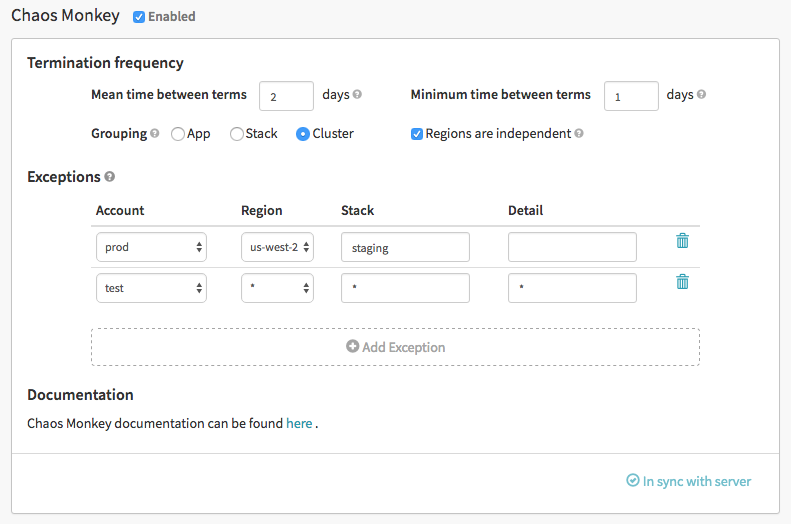
\includegraphics[width=0.9\textwidth]{img/spinnakerconfig.png}
    }
    \label{fig:spinnakerconfig}
\end{figure}

Once Chaos Monkey is set up, some behaviour can be configured in the Spinnaker web UI (see Figure \ref{fig:spinnakerconfig}). This is limited to instance termination frequency, grouping of instances, and the exception of instances \cite{chaosMonkeyManual}.

\subsection{Gremlin}

In December 2017, American company Gremlin Inc. released \textit{Gremlin}, a commercial SaaS\footnote{Software as a Service}-platform allowing organizations to run chaos engineering experiments on their own systems. Gremlin was founded by Kolton Andrus, previous chaos engineer at Netflix, and Matthew Fornaciari, previous senior platform engineer at Salesforce \cite{gremlinAbout}. Gremlin was previously only available at a cost but a free version with limited features is available since February 27, 2019 \cite{gremlinFree}.

While Chaos Monkey only supports the termination of instances, Gremlin features a selection of different types of attacks the user can invoke. These different selections are called \textit{Gremlins}\footnote{Gremlin: A mythical creature reputed to be mischievously inclined to damage or dismantle machinery. (Definition by Wiktionary)}. The different gremlins represent attacks on resources, state, as well as the network \cite{gremlinManual}. For a full list of all available gremlins, see table \ref{tab:gremlins}.

\begin{table}[h]
\centering
\caption {All Gremlins available in Gremlin \cite{gremlinManual}.}
\begin{tabular}{ll}
\multicolumn{2}{l}{\textbf{Resource Gremlins}}                                 \\ \hline
CPU            & Consumes CPU resources                                        \\
Disk           & Consumes disk space                                           \\
IO             & Consumes targeted file system devices resources               \\
Memory         & Consumes memory                                               \\
               &                                                               \\
\multicolumn{2}{l}{\textbf{State Gremlins}}                                    \\ \hline
Process Killer & An attack which kills a specified process                     \\
Shutdown       & Reboots or shuts down the targeted host operating system      \\
Time Travel    & Changes the system time                                       \\
               &                                                               \\
\multicolumn{2}{l}{\textbf{Network Gremlins}}                                  \\ \hline
Blackhole      & Drops all matching network traffic                            \\
DNS            & Blocks access to DNS servers                                  \\
Latency        & Adds latency to all matching egress network traffic           \\
Packet Loss    & Introduces packet loss to all matching egress network traffic
\end{tabular}
\label{tab:gremlins}
\end{table}

While Chaos Monkey works by installing Chaos Monkey on a Spinnaker server, Gremlin works in a completely different way. As a hosted SaaS, Gremlin hosts a web app client for executing Gremlin attacks on the instances of your system. To enable this client to control your instances and run attacks, the Gremlin daemon will have to be installed on each instance you want to be able to attack. This daemon is available for a wide variety of Linux distributions including Ubuntu, Debian, and Redhat, as well as cloud platforms Google Cloud Platform and Amazon Elastic Compute Cloud \cite{gremlinManual}. Once the daemon is installed, it has to be initialized by running and entering a \textit{Team ID} and \textit{Secret Key} found in the web client interface, connecting the daemon to the web interface of your team. Gremlin also supports Kubernetes clusters where the daemon can be installed using Helm\footnote{A package manager for Kubernetes. \url{https://helm.sh/}} \cite{gremlinKubernetes}. When an instance is running a correctly configured instance of the Gremlin daemon, the instance will appear in the web interface as a possible target for attacks \cite{gremlinManual}.

\begin{figure}[h]
    \caption{Choosing hosts to attack in the Gremlin web interface.}
    \centering
    \fbox{
        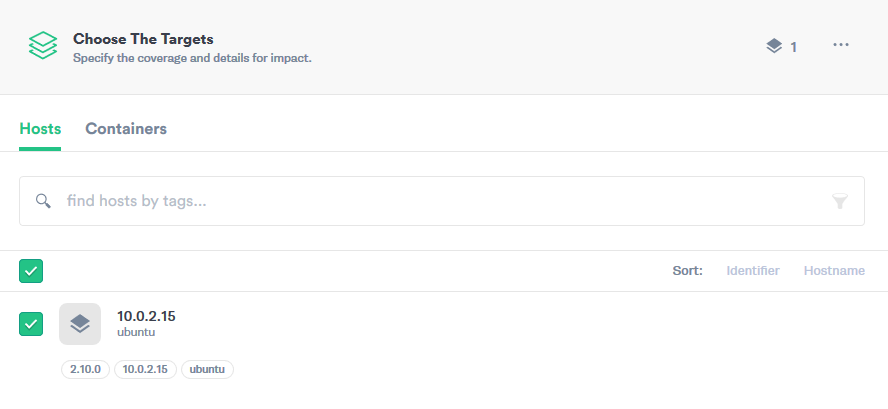
\includegraphics[width=0.9\textwidth]{img/gremlintargets.png}
    }
    \label{fig:gremlinTargets}
\end{figure}

\begin{figure}[h!]
    \caption{Attack type selection in the Gremlin web interface. (Notice how only a subset of attacks are available in the free version)}
    \centering
    \fbox{
        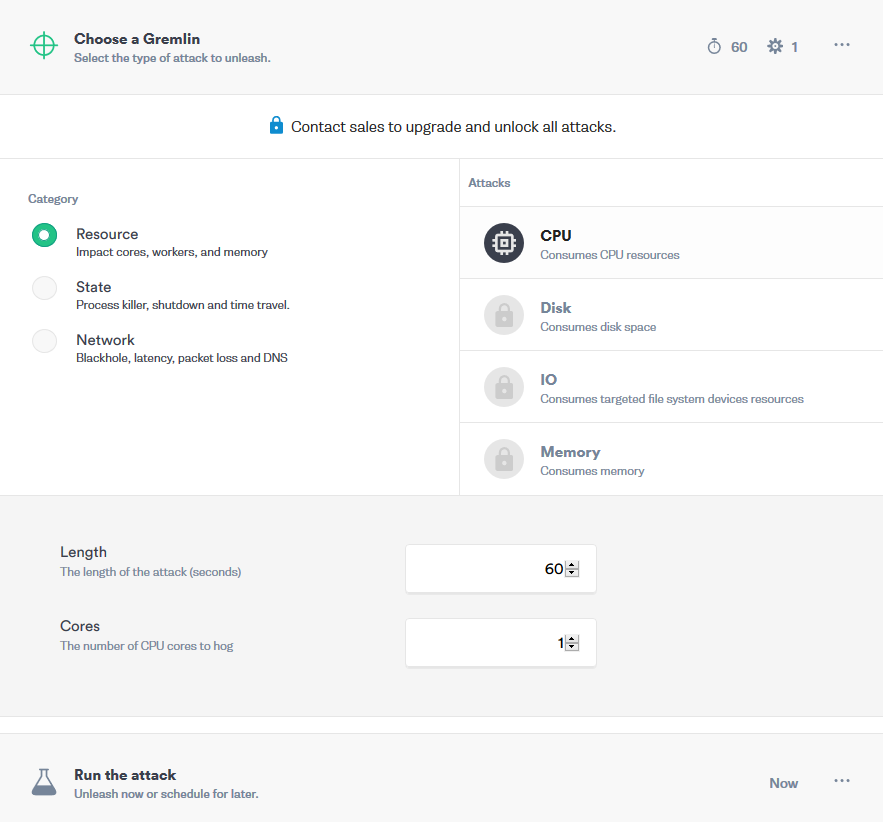
\includegraphics[width=0.9\textwidth]{img/gremlinattacks.png}
    }
    \label{fig:gremlinAttacks}
\end{figure}

To orchestrate an attack in Gremlin, the user chooses a selection of hosts or pods and containers, in the case of a Docker containers or a Kubernetes cluster, to attack (as seen in figure \ref{fig:gremlinTargets}). An option is also available that lets Gremlin pick hosts at random. Once hosts have been selected, the type of attack is chosen (as seen in figure \ref{fig:gremlinAttacks}). As previously mentioned, there exists a variety of different ''Gremlins'' to unleash on the chosen hosts as seen in table \ref{tab:gremlins}. The attacks also come with some options for configuration. These options differ between different types of attack. For example, the CPU attack allows the user to choose the duration of the attack as well as the amount of cores to affect. Finally, there's the choice of executing the attack immediately or to schedule it for later. Scheduling has the option of setting a precise date and time for the attack or to execute it at a random time within a given timeframe. As with Chaos Monkey, there is also the option of invoking an attack from the command line. However, this will only affect the host on which the command is run \cite{gremlinManual}. Whenever attacks are running, Gremlin allows the user to halt them all with a single button. This feature also reverts any changes made to the host as part of the attacks.

Once an attack has been executed, the attack is logged in the web app. Details include but are not limited to the time and duration of the attack, the duration, as well as whether it was carried out successfully or an error was encountered. However, it does not include any information regarding how your system was affected. Gremlin does not include any monitoring tools and it is up to the user to monitor his systems to study the effects of the attack.

\section{Discussion}
\label{sec:discussion}

In this section, we elaborate on our own personal thoughts regarding chaos engineering in general, and the tools presented in section \ref{sec:stateoftheart} in particular.

\subsection{Adoption \& Spread}
Many of what could be considered today's ''tech giants'' are known to be using various forms of chaos engineering to increase the stability of their systems. Chaos Monkey was created at Netflix and the Gremlin founders both have previous experience working at system reliability at Amazon \cite{gremlinAbout}.

In a 2016 interview with Forbes magazine, Jay Parikh, Facebook’s vice president and head of engineering and infrastructure, claims that Facebook started working on a project for \textit{''stress-testing the entire network in case one or more data centers or regions went dark``} \cite{forbes}.

It is also not just software companies using chaos engineering practices. Gremlin presents a number of customers on their website including Walmart, Under Armour, and Siemens \cite{gremlin}.

\subsection{Accessibility \& Usability}
During research for this essay, we tried installing and using both Chaos Monkey and Gremlin. We found Chaos Monkey very hard to set up due to not very detailed documentation, as well as the dependency on Spinnaker. An example Kubernetes cluster running an example quiz web app was deployed using Microsoft Azure, but we did not manage to install and run Chaos Monkey. We found the process cumbersome and the documentation hard to follow. Ironically, we found the Gremlin website to have more easily understandable documentation on Chaos Monkey than the official Chaos Monkey documentation \cite{chaosMonkeyGuide}.

We thought Gremlin was very intuitive to use. After registering a free Gremlin account, an Ubuntu 16.04 virtual machine was set up and the installation instructions for Ubuntu 16.04 were followed. We encountered no issues during installation. We tried running the two attacks available in the free version on our Ubuntu host which worked without issues. We could monitor the CPU usage spiking and we could shut it down remotely from the Gremlin web app. The Gremlin documentation was found extremely detailed, thorough, and easy to read and understand. Furthermore, Gremlin hosts a Gremlin community site which hosts community-made content such as tutorials and talks. In addition to this, Gremlin has it's own YouTube channel with webinars and talks on chaos engineering in general and Gremlin in particular \cite{gremlinYouTube}. Overall we are very impressed with the level of documentation and community content for Gremlin.

Regardless of our issues with installing Chaos Monkey, it is worth mentioning that Chaos Monkey is fully open-sourced and as such all features were available to us at no cost. Gremlin on the other hand required us to sign up for an account to allow us to use the free version. This version was severely limited in that it only allowed for two types of attacks and did not allow for more than one ''team'', in their interface. At the same time, Chaos Monkey only features the shutdown of instances so in that way, the free version of Gremlin still had more options.

\subsection{Final Thoughts}
During our work on this essay we have found the topic of chaos engineering very interesting and a very promising field for the future. With 70\% of companies already having moved to the cloud and 16\% planning to move \cite{GremlinPaper}, the stability of the cloud has become an essential part of our society's infrastructure. The advancement of massive distributed systems on a global scale has added a new level of complexity to this infrastructure and we believe chaos engineering is a natural path forward in building stability and trust in theses systems.

\clearpage

\bibliographystyle{unsrtnat}
\bibliography{references}

\end{document}
